% --- Verzeichnisse ------------------------------------------------------
\newpage
\chapter{Abbildungen}

\begin{figure}[htbp]
    \centering 
		        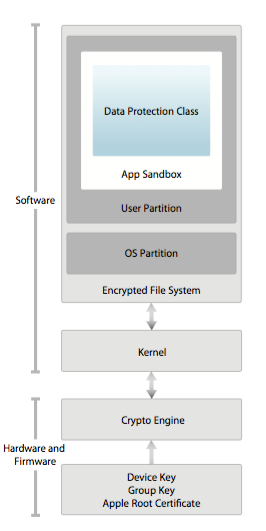
\includegraphics[scale=0.6]{Bilder/SecArchitektur-iOS7.png}
	\caption {iOS Security Architektur iPhone 5c (\cite{Apple[9]} S.3)}
    \label{fig:iOSSecurityArchitekturiOS7}
\end{figure}

\begin{figure}[htbp]
        \centering
                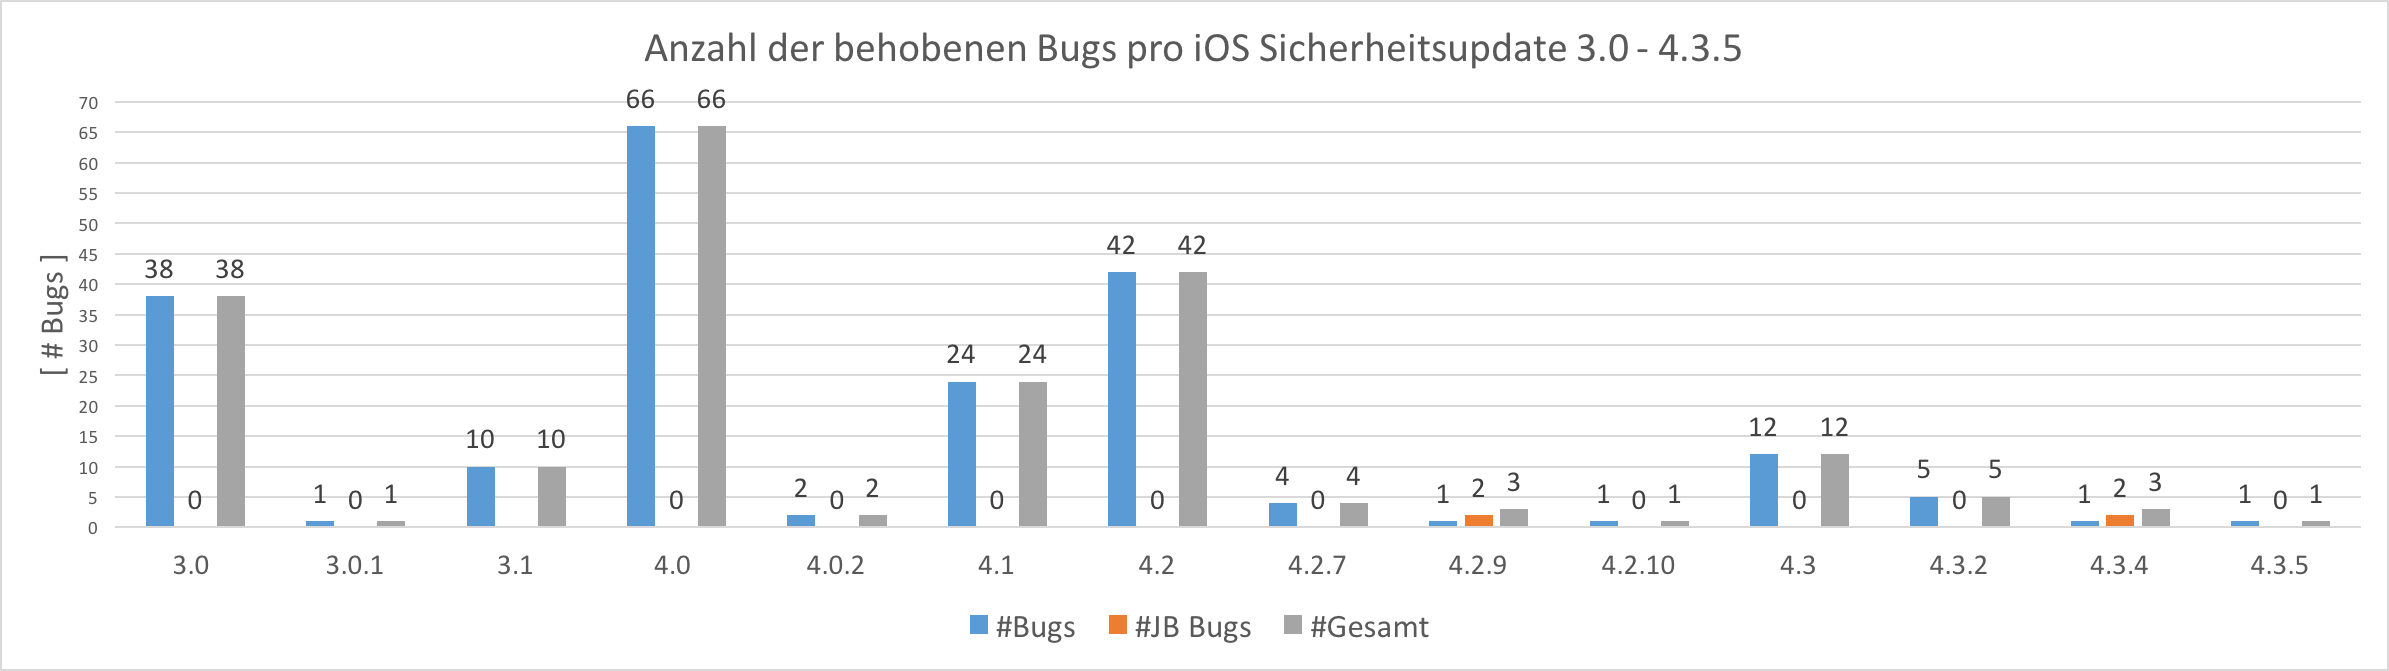
\includegraphics[scale=0.4]{Bilder/iOSSicherheitsupdate3.png}
        \caption{Anzahl Bugs iOS-Sicherheitsupdate iOS Version 3.x - 4.x}
        \label{fig:AnalyseiOSSicherheitsupdate3}
\end{figure}
     
\begin{figure}[htbp]
        \centering
                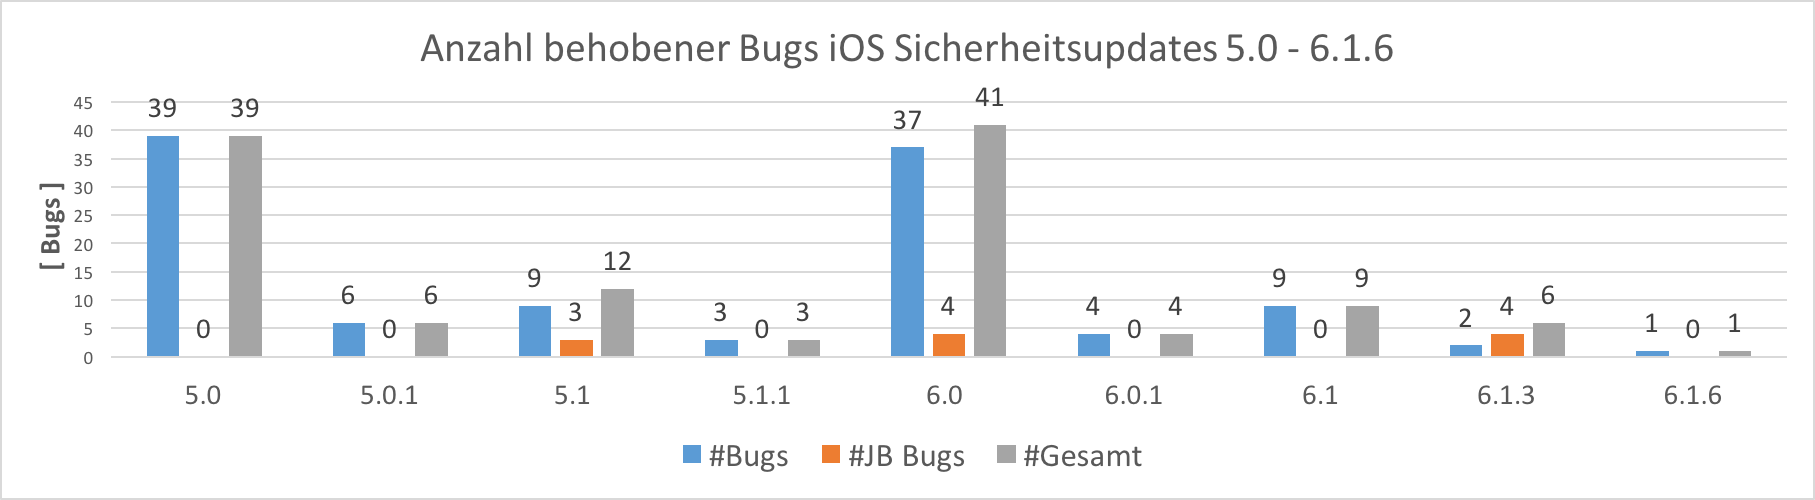
\includegraphics[scale=0.55]{Bilder/iOSSicherheitsupdate5.png}
        \caption{Anzahl Bugs iOS-Sicherheitsupdate iOS Version 5.x - 6.x}
        \label{fig:AnalyseiOSSicherheitsupdate5}
\end{figure}

\begin{figure}[htbp]
        \centering
                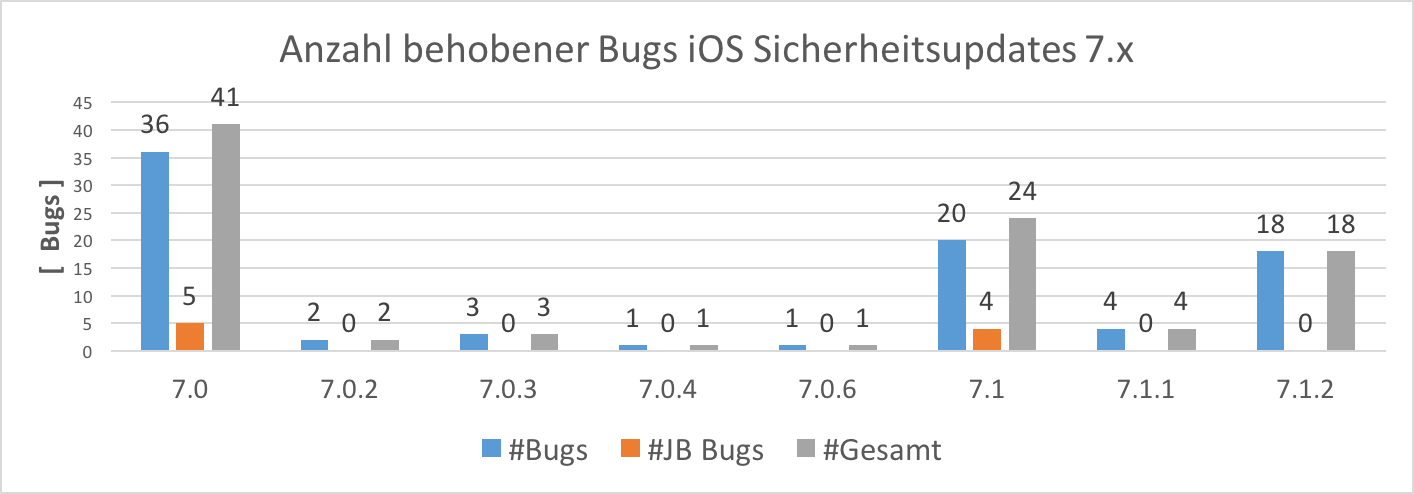
\includegraphics[scale=0.7]{Bilder/iOSSicherheitsupdate7.png}
        \caption{Anzahl Bugs iOS-Sicherheitsupdate iOS Version 7.x}
        \label{fig:AnalyseiOSSicherheitsupdate7}
\end{figure}

\begin{figure}[htbp]
        \centering
                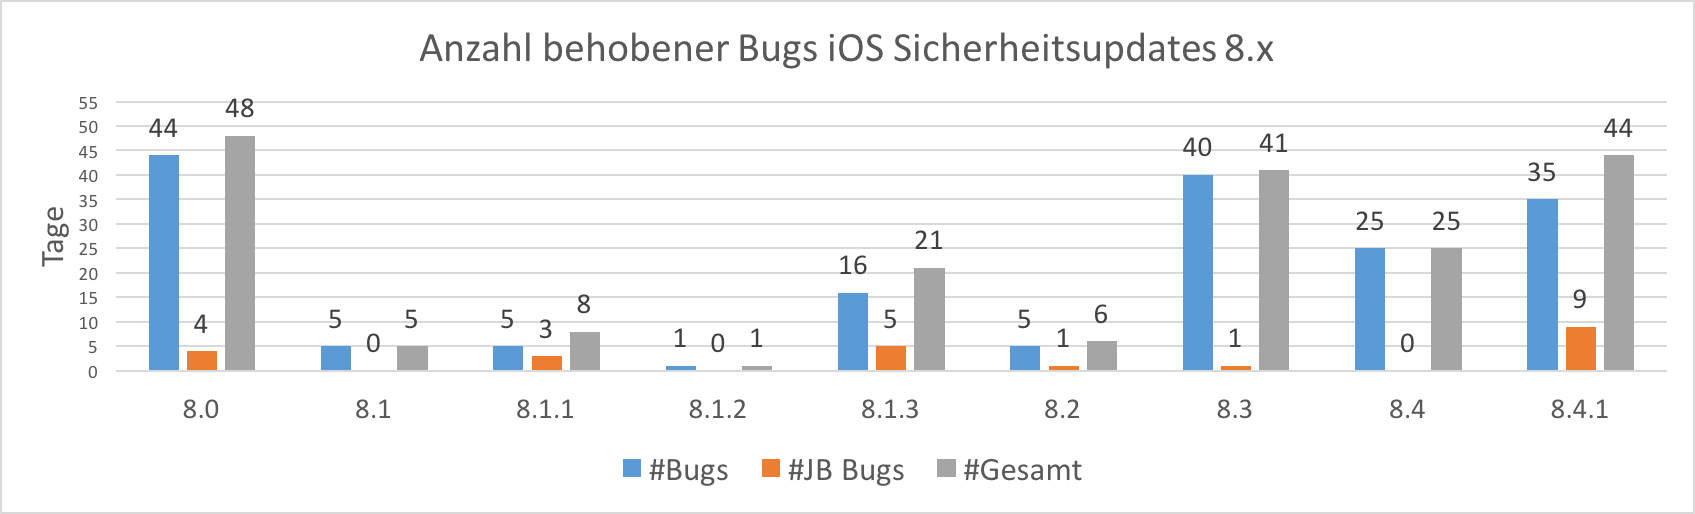
\includegraphics[scale=0.6]{Bilder/iOSSicherheitsupdate8.png}
        \caption{Anzahl Bugs iOS-Sicherheitsupdate iOS Version 8.x}
        \label{fig:AnalyseiOSSicherheitsupdate8}
\end{figure}

\begin{figure}[htbp]
        \centering
                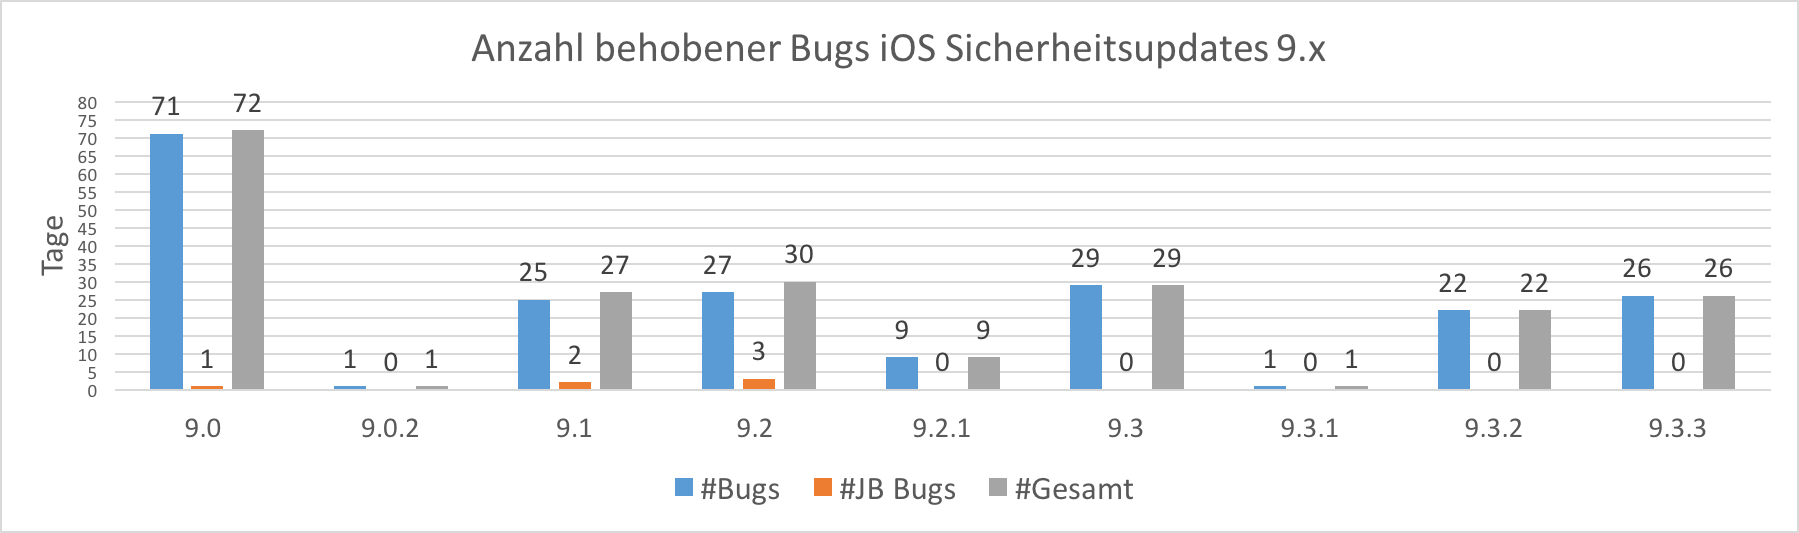
\includegraphics[scale=0.55]{Bilder/iOSSicherheitsupdate9.png}
        \caption{Anzahl Bugs iOS-Sicherheitsupdate iOS Version 9.x}
        \label{fig:AnalyseiOSSicherheitsupdate9}
\end{figure}


\newpage
\chapter{Tabellen}
\begin{table}[htp!]
    \begin{center}
        \begin{tabular}{| p{8mm} | p{18mm} | p{18mm} | p{15mm} | p{15mm} | p{15mm} | p{15mm} | p{15mm} | p{15mm} |} \hline
\textbf{iOS} & \textbf{Samsung S5L8900} & \textbf{Samsung S5L8920} & \textbf{Apple A4}	& \textbf{Apple A5}	& \textbf{Apple A6} & \textbf{Apple A7} & \textbf{Apple A8} & \textbf{Apple A9} \\ \hline
1.0 & iPhone & - & - &  - &  - & - &  - & - \\ \hline		
2.0 & iPhone 3G & - & - &  - &  - & - &  - & - \\ \hline				
3.0 & - & iPhone 3GS & - &  - &  - & - &  - & -	\\ \hline			
4.0 & - &  - & iPhone 4	 &  - &  - & - &  - & -	\\ \hline		
5.0 &  - & - &  - &	iPhone 4s &  - & - &  - & - \\ \hline		
6.0 &  - &  - & - &  - & iPhone 5 & - &  - & -	\\ \hline	
7.0 &  - &  - & - &  - & iPhone 5c	& - &  - & - \\ \hline	
7.0 & - &  - &  - & - &  - & iPhone 5s &  - & - \\ \hline
8.0 & - & - &  - &  - & - &  - & iPhone 6 & - \\ \hline
8.0 & - & - &  - &  - & - &  - & iPhone 6 Plus & -\\ \hline
9.0 & - & - &  - &  - & - &  - & - & iPhone 6s \\ \hline
9.0 & - & - &  - &  - & - &  - & - & iPhone 6s Plus \\ \hline
9.3 & - & - &  - &  - & - &  - & - & iPhone SE \\ \hline     
        \end{tabular} 
        \caption{AuflistungProzessor / iOS Version / iDevice  }
        \label{tab:AuflistungProziOSVersioniDevice}
    \end{center}
\end{table}




